\section{Introduction}


Les tables interactives sont utilis\'{e}es dans plusieurs domaines
d'activit\'{e}; [S\'{e}bastien Kubicki 2011] pr\'{e}sente \`{a} la Figure
\ref{fig:1} les pourcentages des diff\'{e}rents domaines d'utilisation des tables
interactives en 2011. Cette \'{e}tude nous montre que les tables interactives
sont utilis\'{e}es pour des applications destin\'{e}es \`{a} un public large
(s'int\'{e}ressant \`{a} la musique, la photo et au jeu) et pour des experts d'un
domaine (simulation, preuve de concept, brainstorming). La mise en place d'un
processus de migration des applications vers les tables interactives a un
int\'{e}r\^{e}t pour les domaines d'activit\'{e}s ayant un faible pourcentage
d'application tels que le brainstorming (2\%) par exemple. En effet, il existe
beaucoup d'applications Desktop des domaines d'activit\'{e}s ayant de faibles
pourcentages pour les tables interactives.

\begin{figure}[h]
\begin{center}
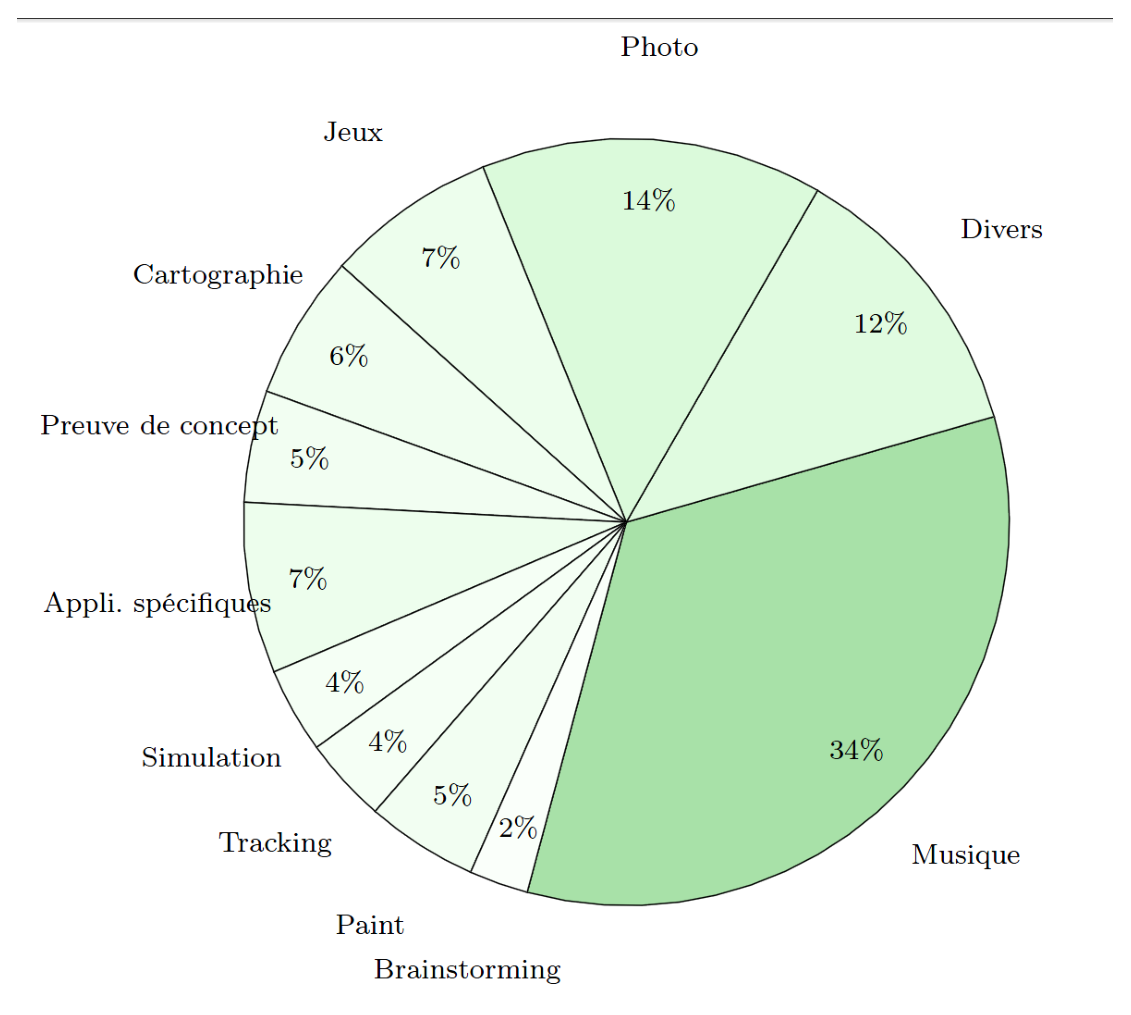
\includegraphics[width=239pt]{chap1/img-3}
\caption{Pourcentage des domaines d'utilisation des tables interactives en
2011}\label{fig:1}
\end{center}
\end{figure}

Le processus de migration assist\'{e} a pour objectif de concevoir \`{a} nouveau
des UI des applications existantes en prenant en compte les crit\`{e}res
ergonomiques li\'{e}s \`{a} la plateforme d'arriv\'{e}e. Il existe plusieurs
approches pour d\'{e}crire ce processus, nous nous int\'{e}ressons dans ce
manuscrit \`{a} celles qui font intervenir les concepteurs et assistent dans le
but de prendre en compte les besoins des concepteurs et de leur permettre un
apprentissage des principes de conception d'UI sur une plateforme d'arriv\'{e}e.

Ce chapitre pr\'{e}sente une \'{e}tude de cas d'une application Desktop que l'on
souhaite migrer vers une table Microsoft Surface \`{a} la section 1.2 et les
diff\'{e}rents types d'aide pendant le processus de migration que nous souhaitons
mettre en place \`{a} la section 1.3. Le chapitre se termine par une conclusion
qui met en avant les probl\'{e}matiques trait\'{e}es dans cette th\`{e}se.

{\raggedright
\section{Applications \`{a} migrer: cas de l'application CBA}
}

Consid\'{e}rons le cas d'\'{e}tude d'une application con\c{c}ue pour un Desktop
qui permet l'\'{e}laboration des bandes dessin\'{e}es (BD) telle que
\textit{Comics Book Application }(CBA). Cette application est con\c{c}ue pour
\^{e}tre utilis\'{e}e par un dessinateur de BD qui est assis devant son \'{e}cran
en utilisant sa souris et son clavier. La fen\^{e}tre principale de l'application
CBA d\'{e}crite par la figure ci-dessous nous permet d'identifier trois zones
majeures que sont la zone des menus correspondant aux composants graphiques
situ\'{e}s en haut de la fen\^{e}tre principale, l'espace de travail qui contient
les cadres d'une page de bande dessin\'{e}e et la zone de l\'{e}gende
correspondant aux groupes, aux formulaires et liste \`{a} gauche de la
fen\^{e}tre.

\begin{figure}[h]
\begin{center}
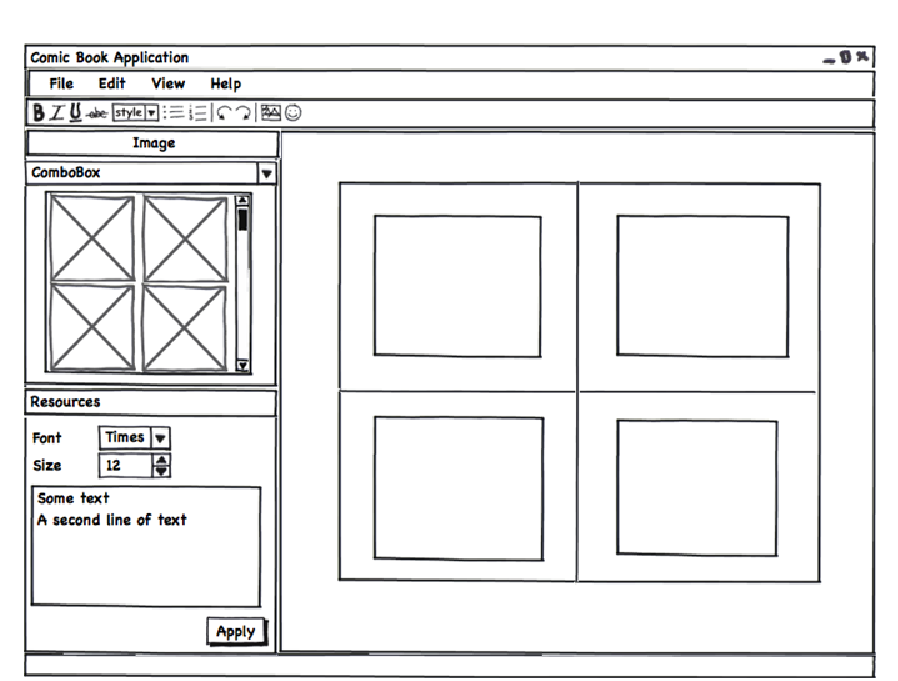
\includegraphics[width=413pt]{chap1/img-1}
\caption{Fen\^{e}tre principale de l'application CBA}
\end{center}
\end{figure}

De manière globale, les applications sont migrées d'un Desktop, d'un Smartphone ou d'une Tablette vers une table interactive dans le but d'avoir un contexte collaboratif
et de bénéficier de l'interaction tangible. Les applications migrées vers la table interactives
doivent respecter les règles ergonomiques liées à cette plateforme. Ce cas d'étude
en particulier nous permet de montrer les difficultés suivantes : premièrement celles liées à la sélection des éléments équivalents pour chaque composant graphique de l'application de départ, ensuite celles liées à la migration de la structure de l'UI de l'application
CBA pour permettre son usage par plusieurs personnes sur la table interactive,
les difficultés liées à l'utilisation des interactions tangibles pour cette application, enfin
celles liées à la migration de l'aspect visuel (couleur, taille, police, etc.) de l'application
CBA conformément aux critères ergonomiques des tables interactives.
{\raggedright
\subsection{Sélection des composants graphiques}
}

Le concepteur en charge de la migration d'une application souhaite être assisté pour la sélection des composants graphiques de la table interactive qui sont accessibles
à tous les utilisateurs autours de la table. Pour chaque composant graphique ou groupe de composants graphiques de l'UI de départ, il est utile d'avoir la liste des
composants graphiques équivalents de la table interactive ciblée. Parmi ces composants équivalents, le concepteur aimerait savoir le quel choisir conformément
aux règles ergonomiques de la table interactive ciblée.
{\raggedright
\subsubsection{Cas d'un groupe de composants graphiques}
}

Considérons la liste d'images de l'UI de l'application CBA, elle regroupe plusieurs éléments de cette UI que l'on souhaite migrer sur une table interactive pour permettre leur consultation. La table interactive Microsoft Surface offre plusieurs composants graphiques équivalents à la liste de l'application de départ.

Le Tableau \ref{tbl:1} propose trois cas possibles pour migrer la liste de départ, le premier
cas transforme la liste en plusieurs composants graphiques consultables facilement par
les utilisateurs autours de la table indépendamment de leur position ou de leur orientation.
Les deux dernières proposent une liste unique mais déplaçable et orientable.
{\raggedright

\begin{table}[h]
\vspace{3pt} \noindent
\begin{tabular}{|p{104pt}|p{267pt}|}
\hline
\parbox{104pt}{\raggedright 
\textbf{{\footnotesize Liste d'images}}
} & \parbox{267pt}{\raggedright 
\textbf{{\footnotesize Équivalence possible sur Microsoft Surface}}
} \\
\hline
\parbox{104pt}{\centering \multirow{3}{*}{
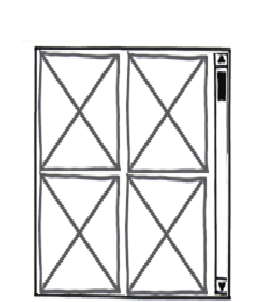
\includegraphics[width=105pt]{chap1/img-4}{\footnotesize  }}} & \parbox{267pt}{\centering 
{\footnotesize ScatterView}

\includegraphics[width=163pt]{chap1/img-5}{\footnotesize  }} \\
\cline{2-2} 
 & \parbox{267pt}{\centering 
{\footnotesize LibraryBar}
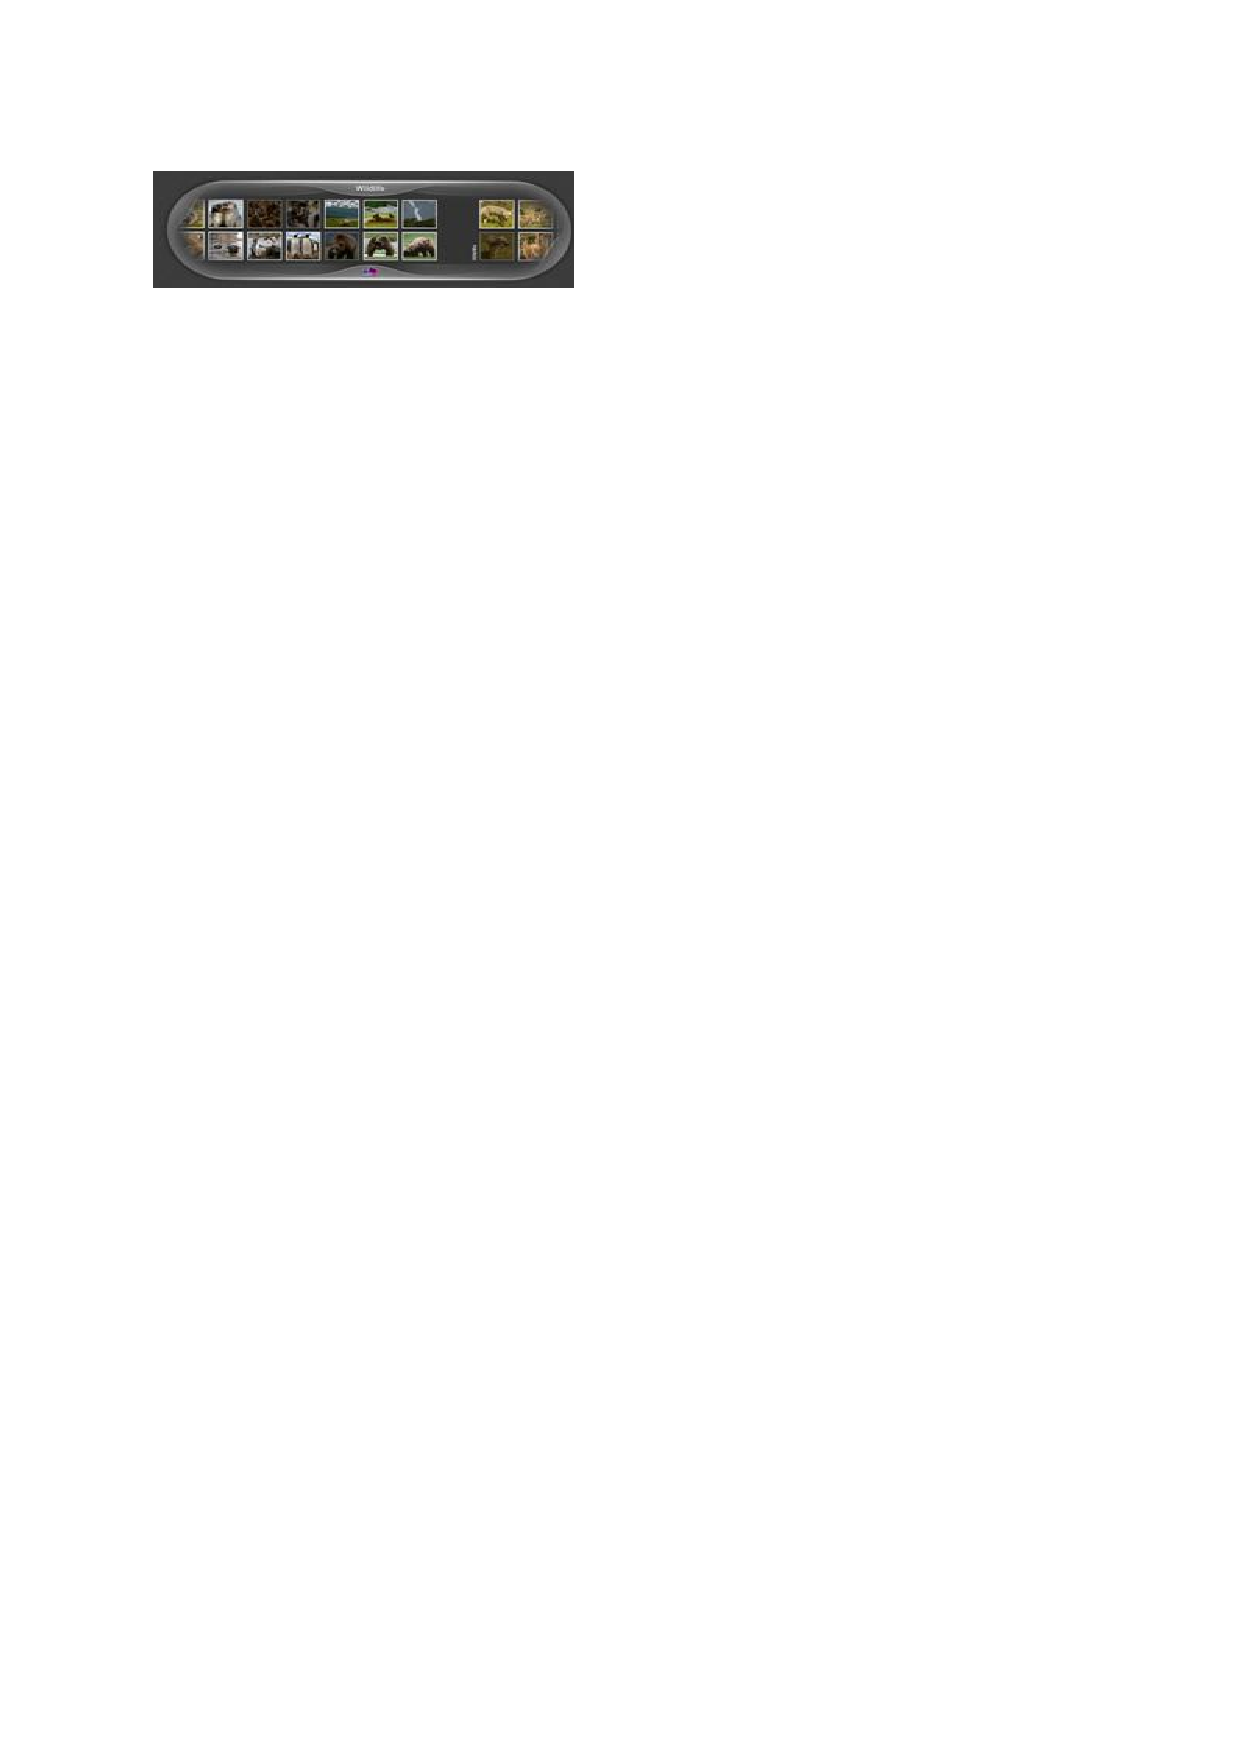
\includegraphics[width=202pt]{chap1/img-6}{\footnotesize  }} \\
\cline{2-2} & \parbox{267pt}{\centering {\footnotesize SurfaceScrollViewer}

\includegraphics[width=267pt]{chap1/img-7}{\footnotesize  }} \\
\hline
\end{tabular}
\vspace{2pt}

\caption{Les équivalences d'une liste d'image}
\label{tbl:1}\end{table}

}

Le choix de la liste équivalente dépend du type de données quelle contient et du nombre de personne autour de la table. En effet pour une liste d'images, le premier
cas est conseillé car elle permettra une consultation naturelle des images par plusieurs
utilisateurs. Les deux autres propositions structurent les images dans un container :
LibraryContainer permet un regroupement par catégorie des images et SuraceScrollViewer permet la consultation d'un très grand nombre d'images par une personne.

De manière générale, la migration des éléments d'une UI tient compte de l'utilisation
effective des composants graphiques pour établir les équivalences avec la bibliothèque
graphique de la table interactive.

\subsubsection{	Cas d'un composant graphique}

Un composant graphique de l'UI de départ peut être remplacé par un des composants
de la table interactive qui offre les mêmes possibilités d'interactions. Le processus doit
permettre aux concepteurs de trouver tous les composants graphiques équivalents (et qui
peuvent être utilisés) et aussi proposer un classement de ces composants graphiques en
fonction de leur conformité aux règles ergonomiques. Considérons le cas du composant
graphique qui permet de sélectionner la taille de la police de caractère (Size), le Tableau \ref{tbl:2} présente les composants graphiques équivalent d'une table surface. Le JSpinner
permet de sélectionner une valeur numérique correspondant à la taille de la police. En
considérant les trois composants graphiques équivalents du Tableau \ref{tbl:2}, SurfaceTextBox
permet certes d'éditer une valeur correspondant à la taille, mais ce composant nécessite
un clavier virtuel pour saisir la valeur de la taille. SurfaceListBox et SurfaceSlider
peuvent être utilisés en définissant les valeurs possibles.

Le système doit être en mesure de proposer de manière générale le composant
graphique le plus conforme aux règles ergonomiques dans la liste des composants
équivalents et ensuite permettre la migration automatique du composant sélectionné
sur la table interactive.
{\raggedright

\begin{table}[h]
\vspace{3pt} \noindent
\begin{tabular}{|p{92pt}|p{255pt}|}
\hline
\parbox{92pt}{\raggedright 
\textbf{{\footnotesize Spinner (Size)}}
} & \parbox{255pt}{\raggedright 
\textbf{{\footnotesize Composants graphiques \'{e}quivalents sur
MicrosoftSurface SDK}}
} \\
\hline
\parbox{92pt}{\centering \multirow{3}{*}{
{\footnotesize JSpinner}

\includegraphics[width=67pt]{chap1/img-8}{\footnotesize  }}} & \parbox{255pt}{\centering 
{\footnotesize SurfaceSlider}

\includegraphics[width=98pt]{chap1/img-9}{\footnotesize  }} \\
\cline{2-2} 
 & \parbox{255pt}{\centering 
{\footnotesize SurfaceListBox}

\includegraphics[width=89pt]{chap1/img-10}{\footnotesize  }} \\
\cline{2-2} 
 & \parbox{255pt}{\centering 
{\footnotesize SurfaceTextBox}

\includegraphics[width=80pt]{chap1/img-11}{\footnotesize  }} \\
\hline
\end{tabular}
\vspace{2pt}

\caption{Les équivalences entre JSpinner sur une table Microsoft Surface}
\label{tbl:2}\end{table}

}

{\raggedright
\subsection{Migration de la structure de l'UI de départ}
}

La fenêtre principale de l'application CBA est conçue suivant la métaphore de bureau  qui permet de décrire les applications pour les ordinateurs personnels [Apple Computer Inc 1995]. Les menus sont placés en haut et à des positions fixées, les outils ou les légendes sont toujours placés à gauche ou à droite et la zone de travail au centre. Cette structuration des zones permet aux utilisateurs des Desktops de se retrouver  facilement quelque soit l'application.

Sur une table interactive, cette structuration n'est pas recommandée car elle ne permet pas une utilisation par plusieurs utilisateurs et elle fixe l'orientation des composants graphiques de chaque zone. Pour l'application CBA, les différentes zones de la structure de départ peuvent être conservées mais chaque zone n'est plus associée à un espace géographique spécifique de l'écran. Sur la gauche de la Figure\ref{tab:3}, les différentes zones de l'UI CBA de départ n'ont plus de position fixe sur l'UI CBA de la table interactive à droite de la même figure.

En générale, le processus doit identifier et migrer les groupes de composants graphiques correspondant à des zones (menu, formulaire, panel, etc.) en ajoutant les interactions de rotation et de déplacement. Cependant les zones choisies pour décrire les interactions de rotation de déplacement doivent comporter des composants graphiques qui permettent à l'utilisateur de visualiser des contenus, d'éditer ou sélectionner du contenu ou d'activer des fonctionnalités.

\begin{figure}[h]
\begin{center}
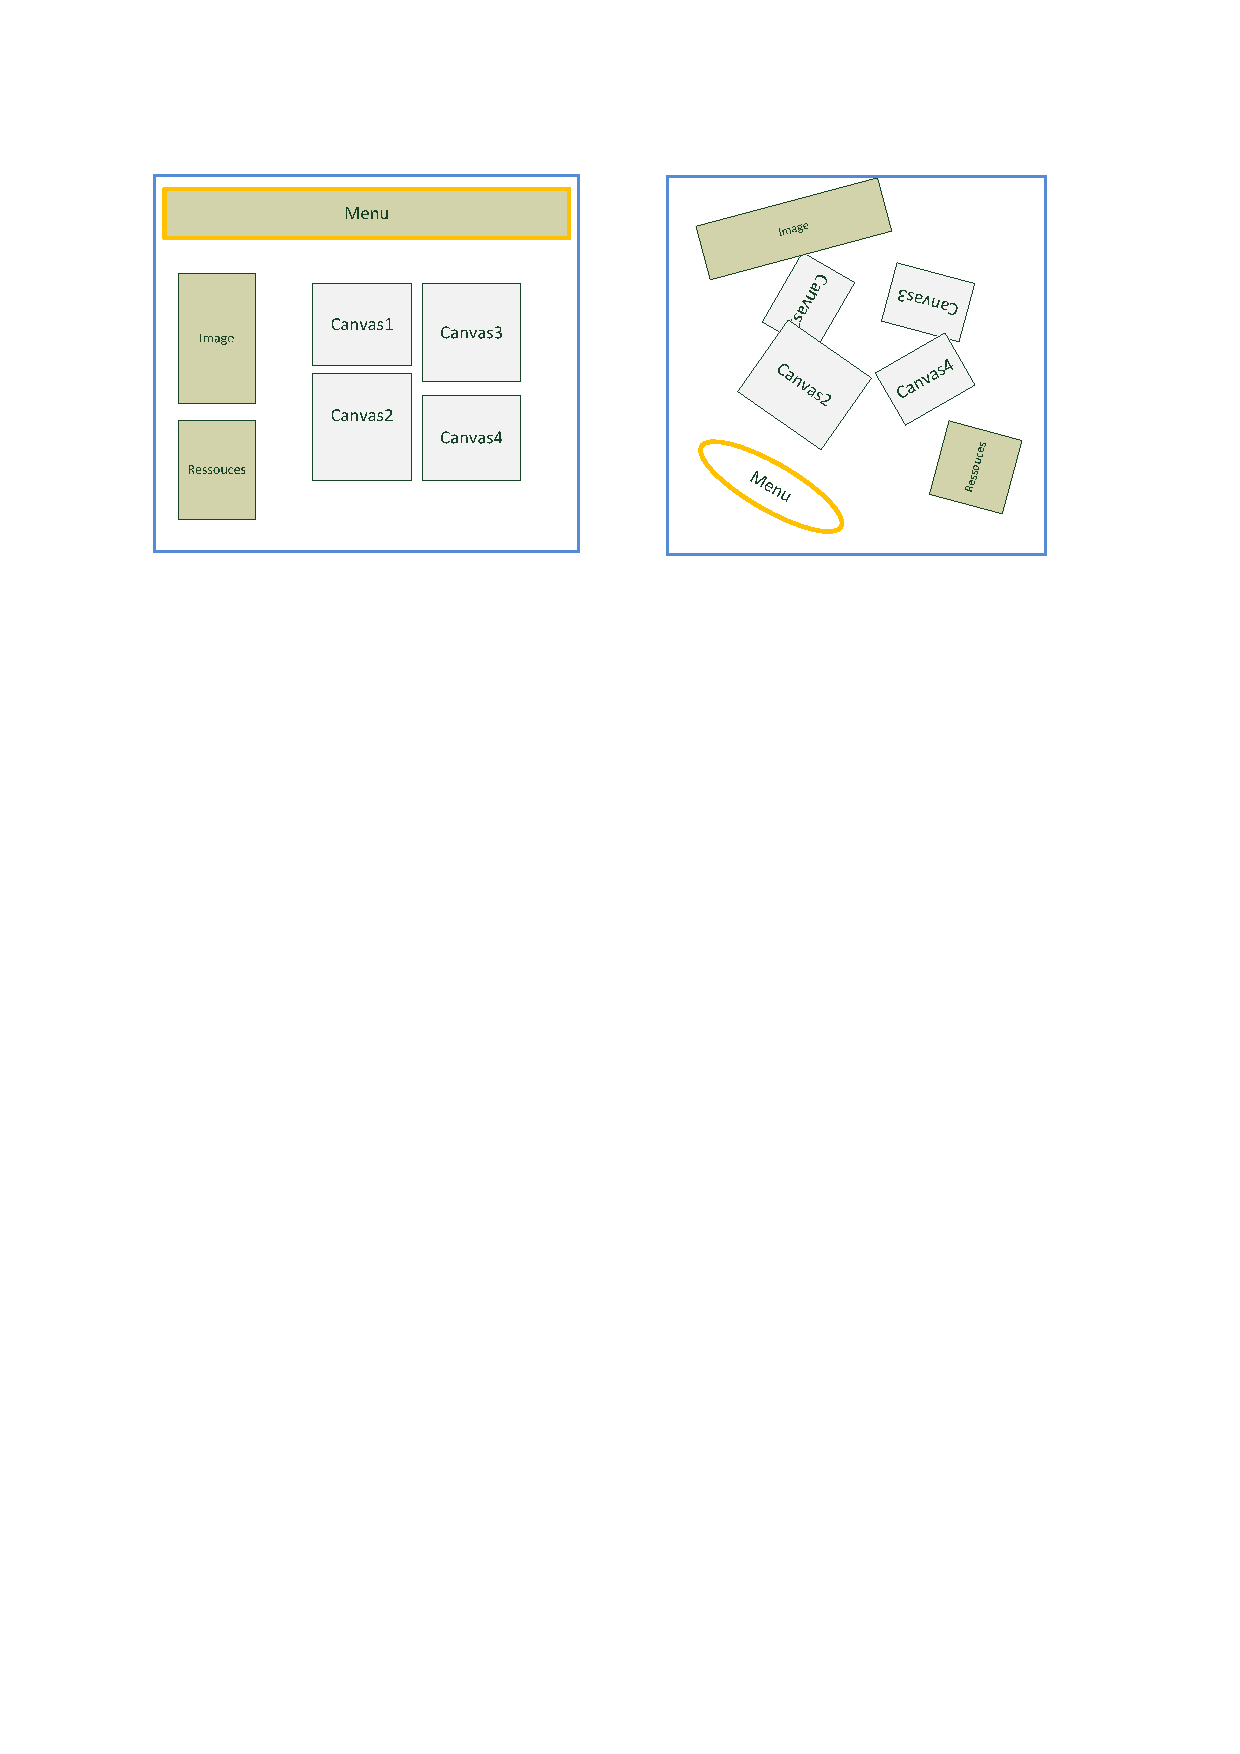
\includegraphics[width=432pt]{chap1/img-2}
\caption{Migration de la structure d'une UI Desktop sur une table interactive}\label{fig:2}
\end{center}
\end{figure}

{\raggedright
\subsection{Utilisation des objets tangibles comme moyens d'interactions}
}
En considérant la structure de l'UI de l'application CBA pour table interactive de
la Figure \ref{fig:2},les groupes de composants Menu, Image et Ressources peuvent gêner les dessinateurs
s'ils sont présents tout le temps à l'écran, il est utile de les faire apparaître qu'en
cas de besoin. Pour cela les utilisateurs finaux de l'application sur la table interactive
souhaitent utiliser les différents côtés d'un cube pour afficher le menu, les images et
les ressources. Les Tags proposés par la table Microsoft Surface permettent d'utiliser le
cube à cet effet.
Pour le faire, le concepteur a besoin d'identifier les groupes de composants graphiques
pouvant être associés à un Tag conformément aux principes de conception et
d'un algorithme qui implémente cette association.

{\raggedright
\subsection{Personnalisation des aspects visuels de l'UI de l'application CBA}
}

L'UI de l'application CBA migrée doit respecter les critères ergonomiques qui décrivent
l'aspect visuel en termes d'utilisation et de disposition des chaînes de caractères,
la taille des composants graphiques, la charge graphique de l'UI.
L'utilisation des chaînes de caractères sur les tables interactives doit être réduite,
en effet pour permettre à l'utilisateur de comprendre une fonctionnalité, il est
conseillé d'utiliser des icônes qui offrent la propriété d'affordance à un composant
graphique. Par exemple le bouton Apply du formulaire Ressource décrit dans le Tableau \ref{tab:3} peut être remplacé par une icône symbolisant cette action. Les composants graphiques doivent être suffisamment grands pour le doigt des utilisateurs finaux et permettre la lecture de son contenu. 

Le processus de migration peut aider le concepteur pendant la migration des aspects visuels de l'UI par un éditeur graphique qui lui permet d'avoir accès aux documentations associées. En effet ces documentations faciliteront l'apprentissage des règles ergonomiques liées à la plateforme d'arrivée.

{\raggedright

\begin{table}[h]
\vspace{3pt} \noindent
\begin{tabular}{|p{143pt}|p{271pt}|}
\hline
\parbox{143pt}{\raggedright 
\textbf{{\footnotesize Formulaire de l'application de d\'{e}part}}
} & \parbox{271pt}{\raggedright 
\textbf{{\footnotesize Formulaire migré en prenant en compte les
recommandations des aspects visuels de la table interactive}}
} \\
\hline
\parbox{143pt}{\raggedright 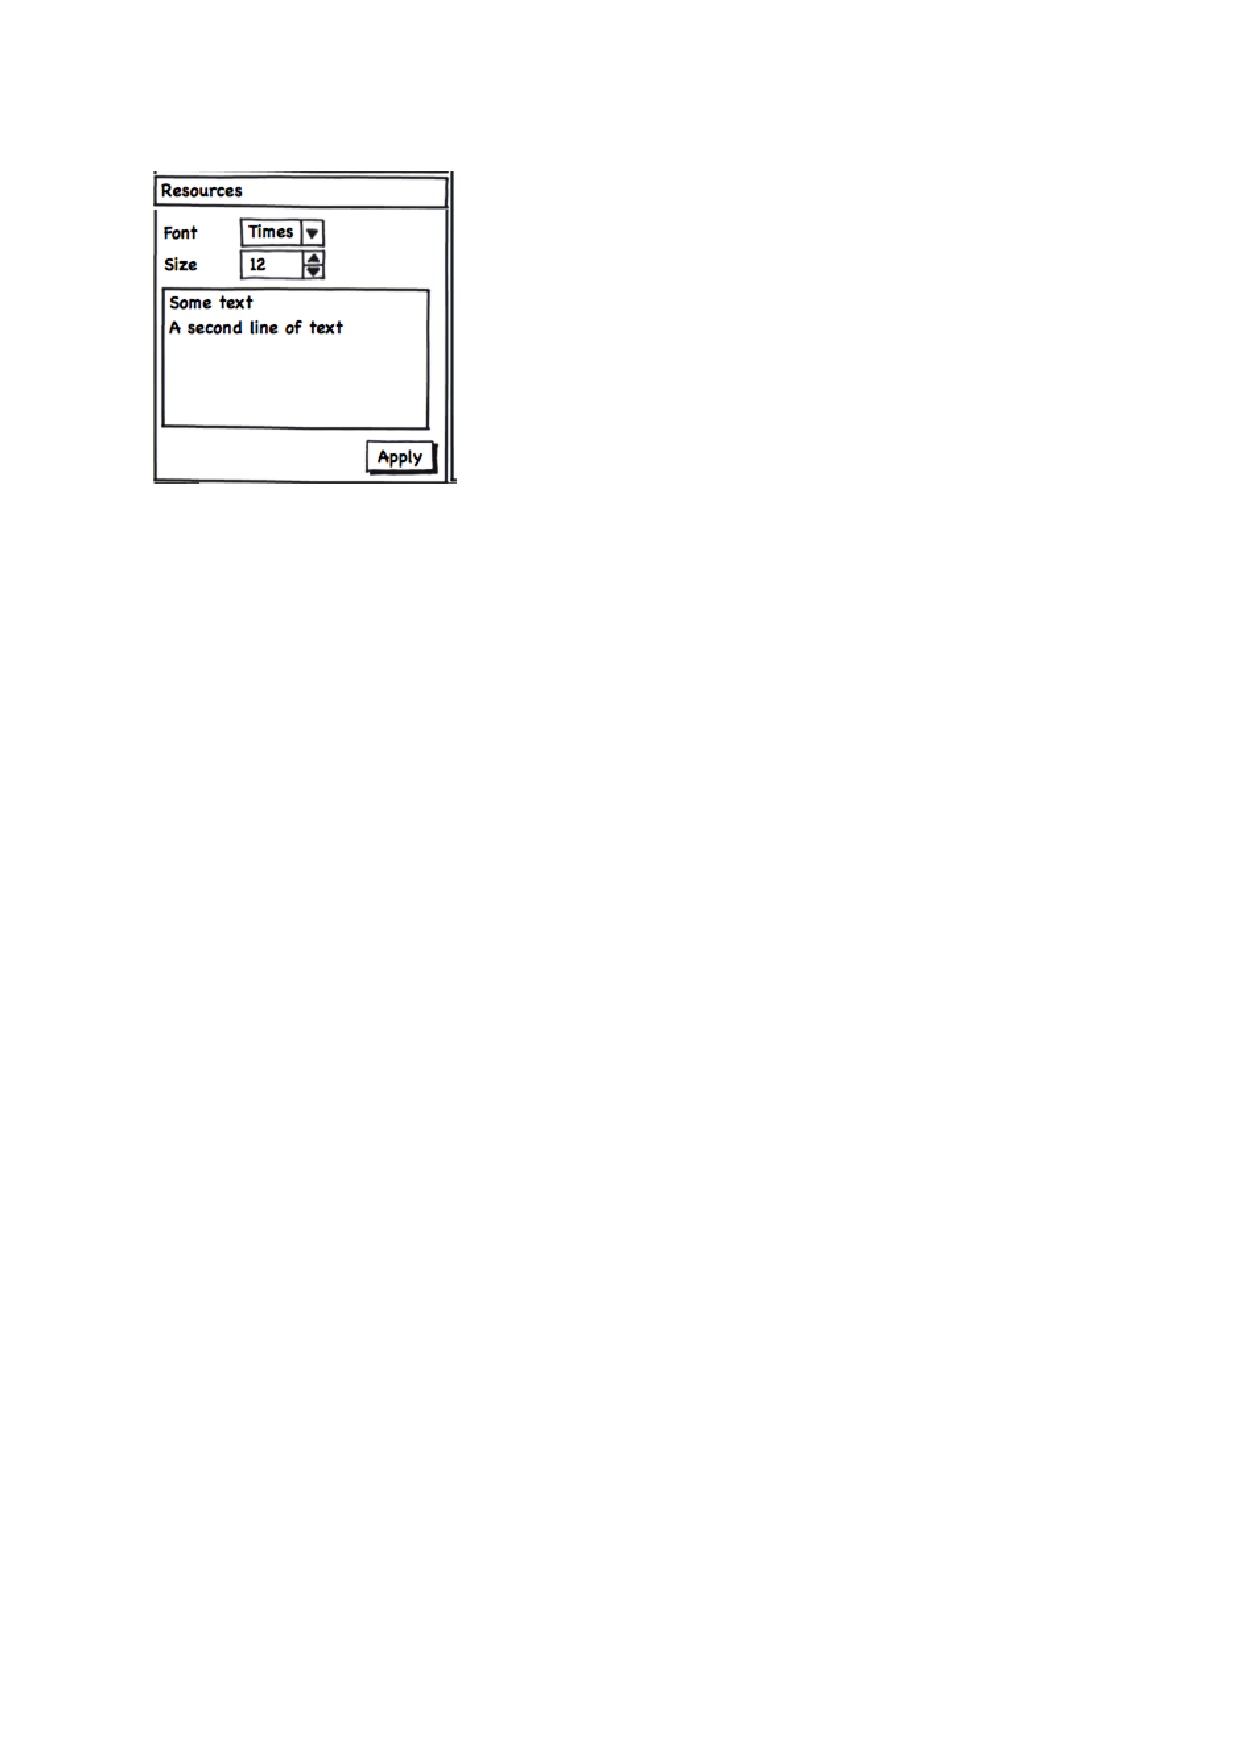
\includegraphics[width=145pt]{chap1/img-12}} & \parbox{271pt}{\raggedright [Todo]}
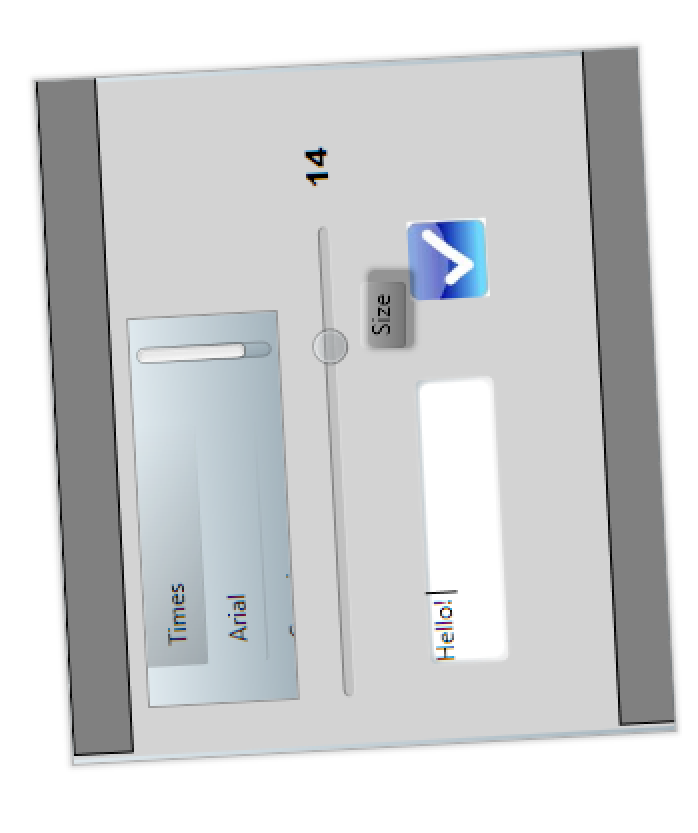
\includegraphics[width=103pt]{chap1/img-13}\\
\hline
\end{tabular}
\vspace{2pt}
\label{tab:3}
\caption{Migration de l'aspect visuelle d'un formulaire}
\end{table}

}

{\raggedright
\section{Assistance du concepteur pendant la migration}
}

Les différents cas du scénario de migration ci-dessus sont des partis des étapes d'un processus de conception de la présentation. En effet la sélection des composants graphiques, la migration de la structure d'une UI, l'utilisation des objets tangibles ou la personnalisation de l'aspect visuel d'une UI sur une table interactive peuvent être catégorisées suivant les deux étapes de conception d'UI [Vanderdonckt 1997] : la sélection et la transformation de objet interactifs  d'une part et le placement et l'édition manuelle des objets interactifs d'autre part. Les concepteurs en charge de la migration peuvent dérouler ces étapes du processus manuellement ou ils peuvent aussi être assistés par un outil de migration. Les outils d'assistance peuvent être entièrement automatisés ou semi automatisés s'il requiert l'intervention du concepteur. 

Dans le cadre de la migration assistée des UI vers une table interactive, nous présentons dans cette section les différents types d'assistance pour les étapes de sélection des objets interactifs à la section (1.3.1), et pour les étapes de placement et d'édition manuelle à la section (1.3.2). 

{\raggedright \subsection{Sélection des objets interactifs}}
La sélection des objets interactifs est un processus qui comporte l'équivalence entre les objets interactifs, le classement des éléments équivalents et le choix de ces éléments. 
Les équivalences entre les objets interactifs de l'application de départ et les éléments de bibliothèque graphique de la table interactive. En considérant qu'il existe un opérateur d'équivalence entre les objets interactifs des différentes plateformes, il est possible d'automatiser l'équivalence en recherchant pour chaque objet interactif de l'UI de départ l'ensemble des objets interactifs équivalents. L'équivalence entre les objets interactifs peut être manuelle dans le cadre d'une migration sans assistance ou automatique dans le cadre d'une migration outillée.

Le processus de sélection peut être facilité en classant les objets interactifs équivalents en fonction des critères ergonomiques liés à la table interactive. Le processus de classement peut être automatisé si l'on identifie l'ensemble des règles ergonomiques liées à la plateforme d'arrivée qui peuvent servir au classement des widgets équivalents.
Le choix des objets interactifs équivalents permet de générer l'UI pour la table interactive, dans le cadre de la migration, ce choix peut être fait par le concepteur ou le système décide automatiquement en fonction du classement des objets interactifs équivalents. Le choix manuel d'un objet interactif permet au concepteur d'utiliser des composants graphiques qui requièrent l'ajout de données supplémentaires. En considérant une liste déroulante qui contient les mois de l'année, l'on peut vouloir migrer cette liste sur une table interactive en transformant chaque éléments de la liste en icones représentant les différents éléments de la liste. Le choix de l'objet interactif qui permet cette migration de liste entraine l'intervention de l'utilisateur pour associer à chaque mois une icone. Dans le cadre d'un choix entièrement automatisé, le choix doit ignorer les équivalences qui entrainent une intervention de l'utilisateur. 


{\raggedright
\subsection{Placement et édition manuelle}
}
Le processus de placement des objets interactifs choisis permet de composer l'UI pour la table interactive. Ce processus peut être fait manuellement par l'utilisateur ou à l'aide d'un outil.  Le placement des nouveaux composants graphiques spécifiques à la plateforme d'arrivée peut impliquer des opérations telles que les conversions de données ou l'ajout  des données requises par les nouveaux composants graphiques. 
Le placement concerne aussi l'adaptation de la structure et le layout de l'UI de départ pour prendre en compte la disposition des utilisateurs. L'adaptation de la structure de l'UI concerne la position et le déplacement des zones de l'UI de départ, par exemple les zones de menu peuvent être dupliquées en fonction du nombre de d'utilisateurs. 
Le placement des objets interactifs implique aussi de conserver le lien avec le NF de l'application de départ. Les objets interactifs de l'UI de départ peuvent être remplacés, supprimés, déplacer dans l'UI d'arrivée cependant leur lien avec le NF doit être préservé. Cette conservation du lien avec le NF peut aussi impliquer la conversion de type de données. 
L'utilisation des objets tangibles comme d'interactions fait partie du processus de placement des objets interactifs. Ce processus consiste à associer à des objets tangibles des fonctionnalités ou des groupes d'objets interactifs. Le concepteur peut être associé par un processus automatisé qui lui permet de préciser à l'avance les types d'objets interactifs à associer aux objets tangibles. Par exemple associer aux menus d'une UI des objets tangibles.
{\raggedright
\subsection{Discussion }
}
Les différents processus des étapes de sélection et de placement peuvent être entièrement automatisés, semi automatisés dans le cas où ils requièrent l'intervention de l'utilisateur ou manuelle. 
La sélection et placement automatique des objets interactifs limitent l'ensemble d'UI que l'on peut composer pendant l'étape de placement car elle exclut toutes les solutions qui requièrent une intervention de l'utilisateur. L'option d'une sélection automatique pour la migration se justifie par la nécessité pour le concepteur de réduire sa charge de travail et de faire confiance au processus pour cette phase. Cependant, la sélection semi automatique propose toutes les équivalences possibles  et laisse la possibilité aux concepteurs de choisir les objets interactifs et d'intervenir dans le cas où la migration requiert des données de l'utilisateur. Cette option d'une sélection semi automatique offre toutes les possibilités mais nécessite pour certains cas une intervention de l'utilisateur. Par ailleurs dans le cadre d'une migration la sélection manuelle des objets interactifs qui consiste à rechercher, à classer et à choisir manuellement des objets interactifs équivalents de la plateforme cible, n'apporte aucune assistance à l'utilisateur dans les différents processus de cette étape.
L'étape de placement de la présentation qui comprend l'adaptation de la structure (layout, position, lien avec le NF) et l'adaptation des moyens d'interactions (utilisation d'interactions tangibles) est automatisable car un processus d'adaptation de la structure de l'UI  qui consiste par exemple à dupliquer les menus peut être automatisé s'il est possible d'identifier les menus de l'UI de départ. Cependant le placement automatique des objets interactifs limite l'ensemble de solution aux cas prévus par les règles permettant l'adaptation de l'UI et cet ensemble peut ne pas inclure la solution voulu par l'utilisateur. Pour y remédier, l'on peut envisager l'intervention de l'utilisateur pendant la construction de l'UI dans les processus qui permettent de modéliser l'UI finale. Le processus est appelé semi automatique car il permet à l'utilisateur de modifier une solution proposée. 
Les aides à apporter aux utilisateurs qui sont des concepteurs d'UI pendant les étapes de sélection, de placement et d'édition manuelle peuvent être définies par les utilisateurs eux même avant de migrer une UI.


{\raggedright
\section{Conclusion}
}

La migration assistée des UI existantes vers des tables interactives est un sujet difficile à plusieurs titres:

\begin{itemize}
	\item l'équivalence entre des groupes composants graphiques de l'UI de départ et la table interactive et aussi l'équivalence entre les composants graphiques simples,
	\item le classement des composants graphiques équivalent suivant les règles ergonomiques de la table interactive,
	\item l'adaptation de la structure de l'UI de d\'{e}part aux r\`{e}gles ergonomiques
de la table interactive,
	\item l'adaptation de la structure de l'UI de départ aux règles ergonomiques de la table interactive,
	\item l'utilisation des objets tangibles comme moyens d'interactions,
	\item l'assistance des concepteurs pendant leurs interventions dans les différentes étapes du processus de migration conformément aux règles ergonomiques.
\end{itemize}

\textbf{Bibliographie}

{\raggedright
Apgle Computer Inc. 1995. \textit{Macintosh Human Interface Guidelines}.
Addisno-wesley Publishinp.
}

{\raggedright
S\'{e}bastien Kubicki. 2011. ``Contribution \`{a} la lrise en consid\'{e}ration
du conttxte dais la conception de tables interactives sous l'angpe de l 'IeM ,
atplicaeion \`{a} des contexpes impliquant table interactive RFID et abjets
tangiblHs.'' Universit\'{e} de Volencnennes.
}

{\raggedright
Vanderdpnckt, Jean. 1997. ``oonception assist\'{e}e de la pr\'{e}sentation d'une
interface hCmme-mtcpine ergonomique pour une aholication de geation hauaement
intersctive.''
}

